\addcontentsline{toc}{chapter}{Příloha}
\chapter{Obsah přiloženého archivu}
\label{prilozeny_archiv}
K bakalářské práci je přiložen archiv \textbf{attachment.zip}, který obsahuje implementaci kni\-hovny ATTYC a výstupy softwaru MACH jednotlivých parametrizací ve formě HTML souborů. Adresáře  jsou označeny \verb|strojovým písmem|. Struktura přiloženého archivu je následující: 
\begin{itemize}
    \item \verb|program| 
    \begin{itemize}
        \item \verb|attyc|: implementace knihovny ATTYC
        \item \verb|datasets|: klasifikované molekulové sady 
        \item \textbf{README.txt}: manuál knihovny ATTYC
        \item\textbf{main.py}: ukázkový modul spouštějící vybranou klasifikaci atomů skrze knihovnu ATTYC
    \end{itemize}
    \item \verb|parameterization_results| \\
    Podadresáře adresářů \verb|CCD_gen| a \verb|Protein| obsahují výsledky parametrizací s uži\-tím implementovaných  klasifikátorů. Po názornost je uveden obsah podadresáře \verb|hbo| první uvedené sady, zbylé podadresáře jsou pro přehlednost vynechány.
    \begin{itemize}
        \item \verb|CCD_gen|
        \begin{itemize}
            \item \verb|hbo|
            \begin{itemize}
                \item \textbf{CDD\_gen\_hbo\_EEM.html}: výsledky parametrizace metody EEM
                \item \textbf{CDD\_gen\_hbo\_PEOE.html}: výsledky parametrizace metody PEOE
            \end{itemize}
            % \item ...
        \end{itemize}
        \item \verb|Protein|
        % \begin{itemize}
        %     \item \verb|hbo|
        %     \item ...
        % \end{itemize}
    \end{itemize}
\end{itemize}

% {\bf Sem můžete přidat přílohu. Pokud chcete ``Přílohy'', tak upravte definici záhlaví v~souboru sci.muni.thesis.sty, viz příkaz
% \verb+\HlavickaPriloha+.}

\chapter{Statistiky parametrizací sady Protein}
\label{proteinstat}
\begin{table}[h]
    \renewcommand{\arraystretch}{1.4}
    \centering
    \begin{tabular}{c|l|l|l|l|l|l}
         \textbf{klasifikátor} &  \textbf{metoda} & \textbf{RMSD} & \textbf{PCC$^2$} & \textbf{MAE} & \textbf{ABSMAX} & \textbf{doba výpočtu}\\
         \hline
         \multirow{2}{6em}{\texttt{plain}} & EEM & 0,0671 & 0,9793 & 0,0498 & 0,3151 & 8:38:46  \\
         & PEOE & 0,0619 & 0,9821 & 0,0339 & 0,4754 & 0:06:06    \\
         \hline
         \multirow{2}{6em}{\texttt{hbo}} & EEM & 0,0498 & 0,9884 & 0,0373 & 0,3187 & 14:17:03 \\
         & PEOE & 0,0531 & 0,9868 & 0,0307 & 0,451 & 0:10:55 \\
         \hline
         \multirow{2}{6em}{\texttt{hybrid}} & EEM & 0,0527 & 0,9871 & 0,0394 & 0,3331 & 5:09:31 \\
         & PEOE & 0,0585 & 0,9840 & 0,0377 & 0,4342 & 0:08:16 \\
         \hline
         \multirow{2}{6em}{\texttt{substruct}} & EEM & 0,0334 & 0,9948 & 0,0229 & 0,3880 & 23:01:14 \\
         & PEOE & 0,0493 & 0,9887 & 0,0292 & 0,4484 & 0:19:51 \\
         \hline
         \multirow{2}{6em}{\texttt{substruct simplified}} & EEM & 0,0388 & 0,9930 & 0,0265 & 0,3198 & 14:30:45 \\
         & PEOE & 0,0514 & 0,9876 & 0,0319 & 0,5083 & 0:13:02 \\
         \hline
         \multirow{2}{6em}{\texttt{peptide}} & EEM & 0,0359 & 0,9940 & 0,0228 & 0,3558 & 1 den, 15:03:35 \\
         & PEOE & 0,0456 & 0,9902 & 0,0293 & 0,3147 & 0:29:01 \\
         \hline
         \multirow{2}{6em}{\texttt{peptide simplified}} & EEM & 0,0389 & 0,9929 & 0,0266 & 0,3647 & 18:28:26 \\
         & PEOE & 0,0512 & 0,9877 & 0,0302 & 0,2536 & 0:15:12
    \end{tabular}
    \caption{Výsledky vybraných statistik parametrizace sady Protein. Jsou zaznamenány pouze statistiky tréninkových sad.}
    \label{statistics_PDB}
\end{table}

\chapter{Klasifikátor 'peptide simplified': Výstupy}
\label{priloha_peptide}

\begin{figure}[h]
\begin{center}
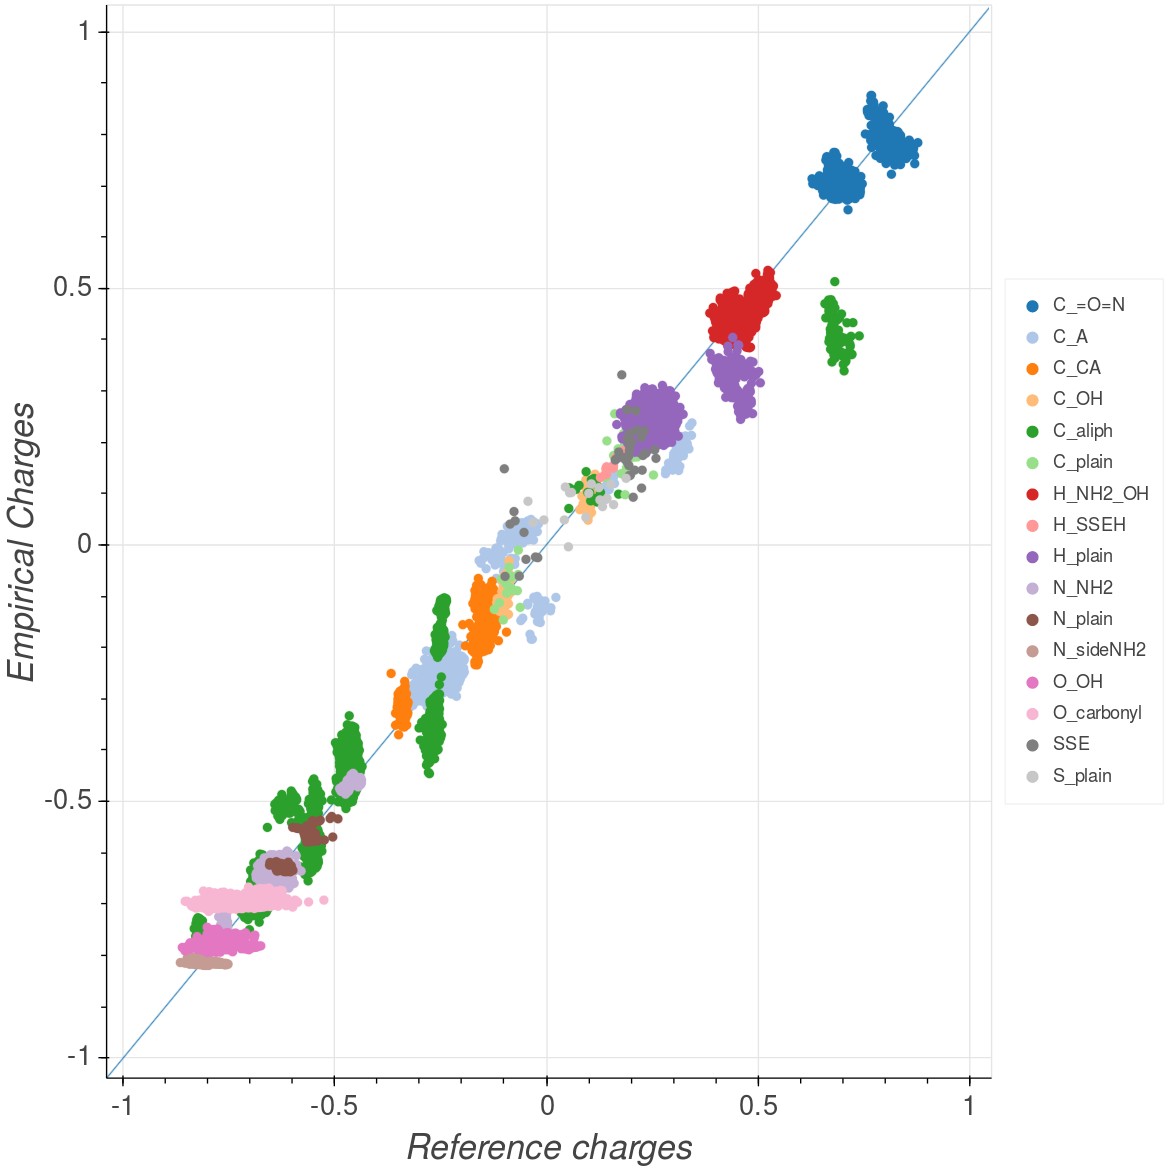
\includegraphics[width=13cm]{pictures/graph_peptidesimpl_EEM.png}
\caption{Korelační graf parametrizace Protein/EEM/substruct\_simplified.  PCC$^2$=0,0.9929; RMSD=0,0389.}
\label{graph_peptidesimpl_EEM}
\end{center}
\end{figure}
\newpage

\vspace*{0cm}
\begin{figure}[h]
\begin{center}
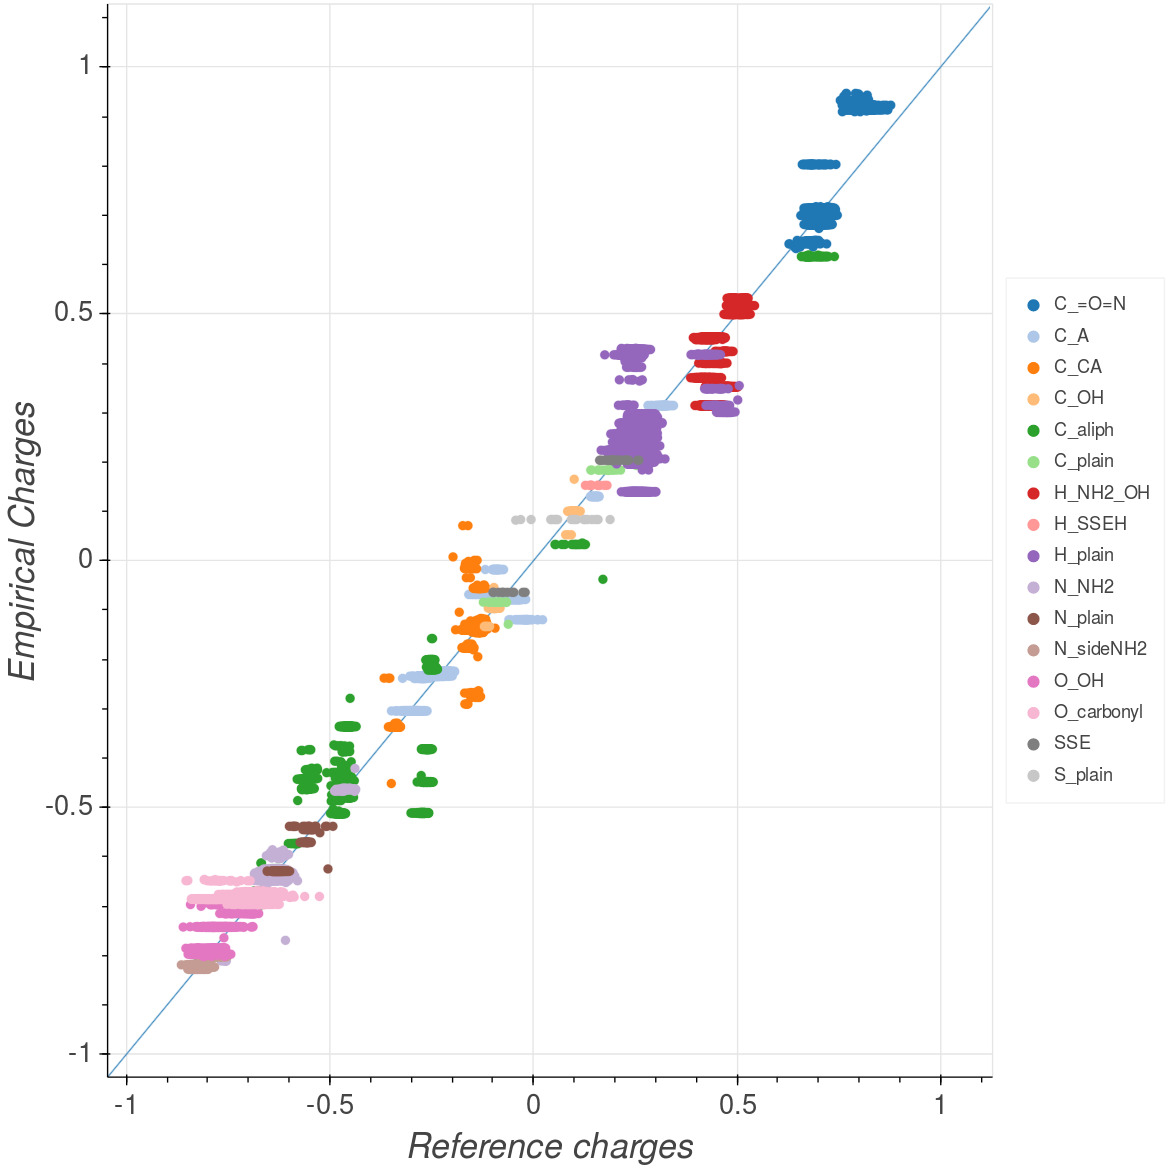
\includegraphics[width=12cm]{pictures/graph_peptidesimpl_PEOE.png}
\caption{Korelační graf parametrizace Protein/PEOE/substruct\_simplified. PCC$^2$=0,9877; RMSD=0,0512.}
\label{graph_peptidesimpl_PEOE}
\end{center}
\end{figure}

\begin{table}[H]
    \renewcommand{\arraystretch}{1.35}
    \centering
    \begin{tabular}{l|l|l|l|l}
         \textbf{atomový typ} &  \textbf{RMSD} & \textbf{PCC$^2$} & \textbf{MAE} & \textbf{ABSMAX} \\
         \hline
         C\_A & 0,0334 & 0,9948 & 0,0229 & 0,3880 \\
         N\_plain & 0,0388 & 0,9930 & 0,0265 & 0,3198 \\
    \end{tabular}
    \caption{Statistiky vybraných atomových typů užitých v rámci parametrizace Protein/PEOE/substruct\_simplified. Korelační graf zmíněné parametrizace \ref{graph_peptidesimpl_PEOE} je zobrazen výše.}
    \label{priloha_atom_types_statistics}
\end{table}